\documentclass[11pt, a4paper]{article}
\usepackage{graphicx}
\usepackage{amsmath}
\usepackage{listings}

\title{Assignment6}
\author{Mudadla Harshavardhan}
\date{March 27, 2022}

\begin{document}

\maketitle % Insert the title, author and date
\section{Time response of a spring}
In this assignment we are about to find output of given function in the s-domain using impulse response of given function.
Consider the forced oscillatory system given by the equation:$x(0)=0,\dot x(0)=0$
\begin{equation}
    \ddot x + 2.25x = f(t)
\end{equation}
where
\begin{equation}
    f(t) = cos(1.5t)e^{-0.5t}*u(t)
\end{equation}
whose laplace transform is
\begin{equation}
    F(s) = (s+0.5)/((s+0.5)^2+2.25)
\end{equation}
Solving for $X(s)$ in Laplace domain we get,
\begin{equation}
    X(s) = \frac{s+0.5}{(s+0.5^2)+2.25)(s^2+2.25)}
\end{equation}
\begin{figure}[!tbh]
  \centering
  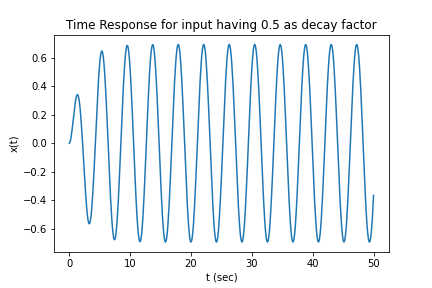
\includegraphics[scale=0.5]{0.5decay.png}
  \caption{x(t) vs t at decay constant 0.5} 
  \label{fig:fig1}
\end{figure} 

\begin{figure}[!tbh]
  \centering
  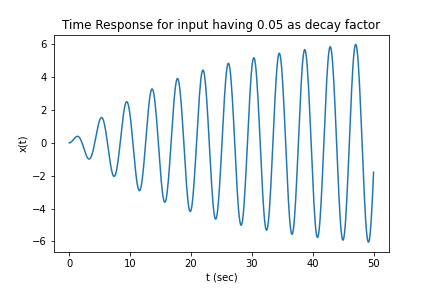
\includegraphics[scale=0.5]{0.05decay.png}  
  \caption{x(t) vs t at decay constant 0.05} 
  \label{fig:fig2}
\end{figure} 
\pagebreak
\newpage
\section{Time response of a spring using transfer function}
Obtain system transfer function $X(s)/F(s)$ for above $x(t),f(t)$. And vary $\omega$ from 1.4 to 1.6 with 0.05 gapping in $f(t)$.Use $signal.lsim$ and find resulting responses and plot them.
From the given equation, we can see that the natural response of the system has the frequency w = 1.5 rad/s . Thus, as expected the maximum amplitude of oscillation is obtained when the frequency of $f(t)$ is 1.5 rad/s, due to resonance.
\begin{figure}[!tbh]
  \centering
  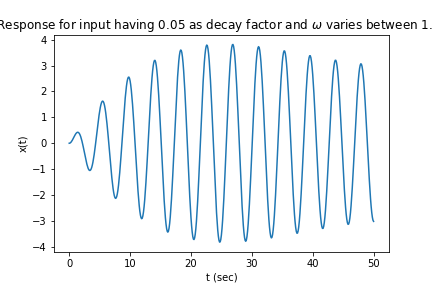
\includegraphics[scale=0.5]{wvary1.4.png}
  \caption{responses at 1.4 frequency} 
  \label{fig:fig3}
\end{figure}
\begin{figure}[!tbh]
  \centering
  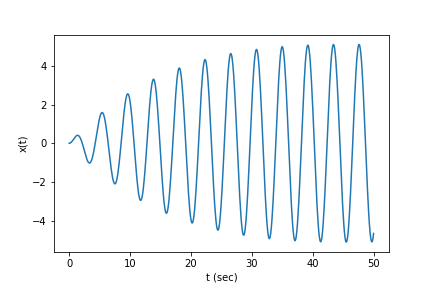
\includegraphics[scale=0.5]{wvary1.45.png}
  \caption{responses at 1.45 frequency} 
  \label{fig:fig4}
\end{figure}
\begin{figure}[!tbh]
  \centering
  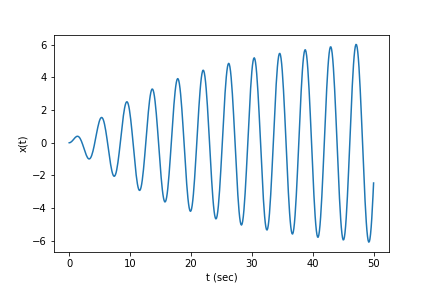
\includegraphics[scale=0.5]{wvary1.5.png}
  \caption{responses at 1.5 frequency} 
  \label{fig:fig5}
\end{figure}
\begin{figure}[!tbh]
  \centering
  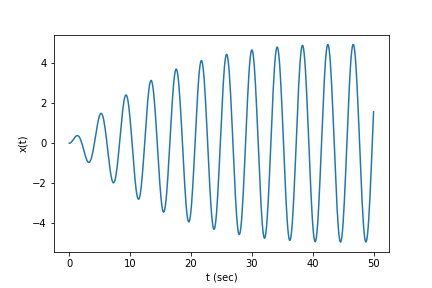
\includegraphics[scale=0.5]{wvary1.55.png}
  \caption{responses at 1.55 frequency} 
  \label{fig:fig6}
\end{figure}
\begin{figure}[!tbh]
  \centering
  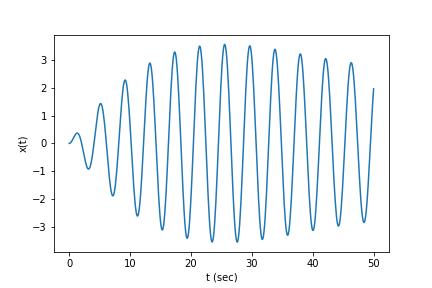
\includegraphics[scale=0.5]{wvary1.6.png}
  \caption{responses at 1.6 frequency} 
  \label{fig:fig7}
\end{figure}
\section{Coupled spring problem}
We now consider a coupled Differential system
\begin{equation}
    \ddot x + (x-y) = 0
\end{equation}
and 
\begin{equation}
    \ddot y + 2(y-x) = 0
\end{equation}
with the initial conditions: $\dot x(0) =0,\dot y(0) =0,x(0) =1,y(0) =0$.
Taking Laplace Transform and solving for $X(s)$ and $Y(s)$, We get:
\begin{equation}
    X(s) = \frac{s^2+2}{s^3 + 3s}
\end{equation}
\begin{equation}
    Y(s) = \frac{2}{s^3 + 3s}
\end{equation}
And with time being constrained between 0 and 20 we need to plot both $x(t),y(t)$ with respect to time.
\begin{figure}[!tbh]
    \centering
    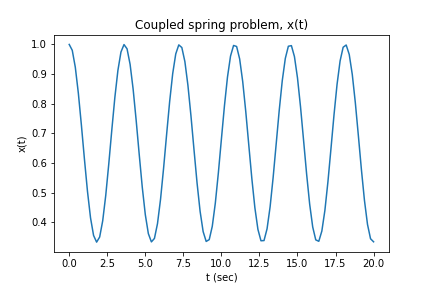
\includegraphics[scale=0.5]{x_t.png}  
    \caption{plot of x_t in coupled spring } 
    \label{fig:fig8}
\end{figure}
\begin{figure}[!tbh]
    \centering
    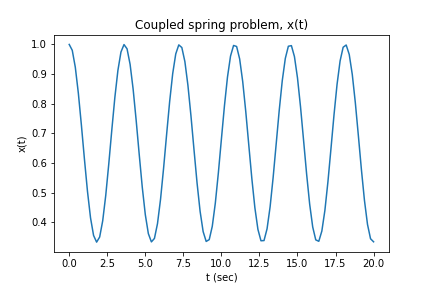
\includegraphics[scale=0.5]{x_t.png}  
    \caption{plot of y_t in coupled spring } 
    \label{fig:fig9}
\end{figure}
\pagebreak
\newpage
\section{Two-port Network}
We need to obtain Magnitude and phase response of the steady state transfer function of given 2 port network.
The Steady-State transfer function of the given circuit is given by
\begin{equation}
    H(s) = \frac{10^6}{s^2/10^6 + 100s + 10^6}
\end{equation}
  \begin{figure}[!tbh]
    \centering
    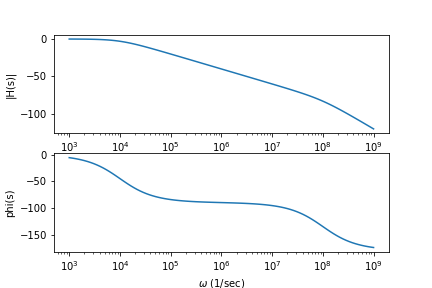
\includegraphics[scale=0.5]{Bodeplot.png}  
    \caption{Magnitude response and phase response} 
    \label{fig:fig10}
  \end{figure}
\section{Low pass filter response}
Low pass filter is given by below equation:\newline
\begin{center}
$V_i(t) = (cos(10^3t) - cos(10^6t))u(t)$
\end{center}
we need to find output for $0<t<30\mu s$ and $0<t<10ms$ using $signal.lsim$ nd then plot it w.r.t input.
we can find all by using $t,y,svec=sp.lsim(H,u,t)$ where y is output, u is input, H is transfer function of given 2 port network.
    \begin{figure}[!tbh]
      \centering
      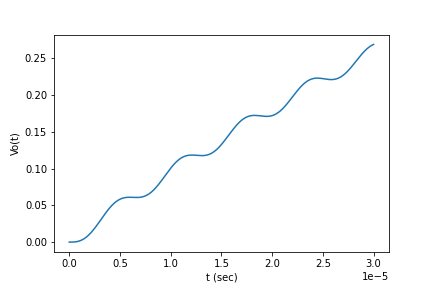
\includegraphics[scale=0.5]{Vo_t1.png}  
      \caption{for $0<t<30\mu s$} 
      \label{fig:fig5}
    \end{figure}
    \begin{figure}[!tbh]
      \centering
      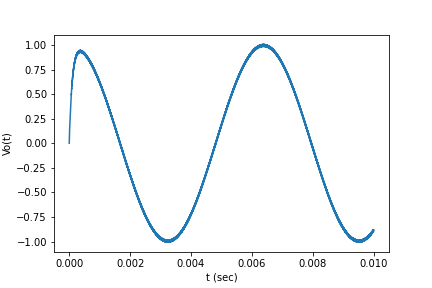
\includegraphics[scale=0.5]{Vo_t2.png}  
      \caption{for $0<t<10ms$} 
      \label{fig:fig6}
    \end{figure}
\section{Conclusion}
    The scipy.signal library provides a useful toolkit of functions for circuit analysis. The toolkit was used for the analysis of LTI systems in various domains.\\
    The forced response of a simple spring body system was obtained over various frequencies of the applied force, and highest amplitude was observed at resonant frequency.\\
    A coupled spring problem was solved using the sp.impulse function to obtain two sinusoids of the same frequency.\\
    A two-port network, functioning as a low-pass filter was analysed and the output was obtained for a mixed frequency input.
\end{document}
